\section{Simulation}
\subsection{Monte Carlo Simulation}
Monte Carlo Simulation ist eine numerische Methode für statistische Simulation, die Sequenzen von Zufallszahlen benutzt, um die Simulation durchzuführen.

\textbf{Eigenschaften:}
\begin{compactitem}
	\item Monte Carlo Simulation ist ein kräftiges Instrument, um komplexe statistische Analysen durchzuführen und Wahrscheinlichkeiten und Verteilungen zu schätzen.
	\item Es verlangt ein Systemmodell (quantitative Systembeschreibung).
	\item Es werden (virtuelle) Experimente mit dem System ausgeführt, um Schlussfolgerungen bzgl. deren Verhalten zu ziehen.
\end{compactitem}

\begin{example}
	Berechne den Wert von $\pi$
	\begin{multicols}{5}
		Fläche Rechteck: $(2r)^2$ \\
		Fläche Kreis: $\pi r^2$ \\
		$\frac{\text{Fläche Rechteck}}{\text{Fläche Kreis}}$: $\frac{4}{\pi}$ \\
		$\pi$: $4 * \frac{\text{Fläche Kreis}}{\text{Fläche Rechteck}}$ \\
		$\pi$: $4 * \frac{\text{Punkte im Kreis}}{\text{Punkte im Rechteck}}$	
	\end{multicols}
	\begin{minipage}[h]{0.825\textwidth}
		\begin{lstlisting}[mathescape=true, tabsize=2]
N Punkte $X_i$ = -1 + 2$A_i$ und
N Punkte $Y_i$ = -1 + 2$B_i$ mit A, B Sequenzen von unabhaengigen Zufallszahlen
K = 0
	for i = 1 : N
		if ($X_i^2$ + $Y_i^2$ < 1)
			K = K + 1
		end
end
		\end{lstlisting}
	\end{minipage}
	\begin{minipage}[h]{0.175\textwidth}
		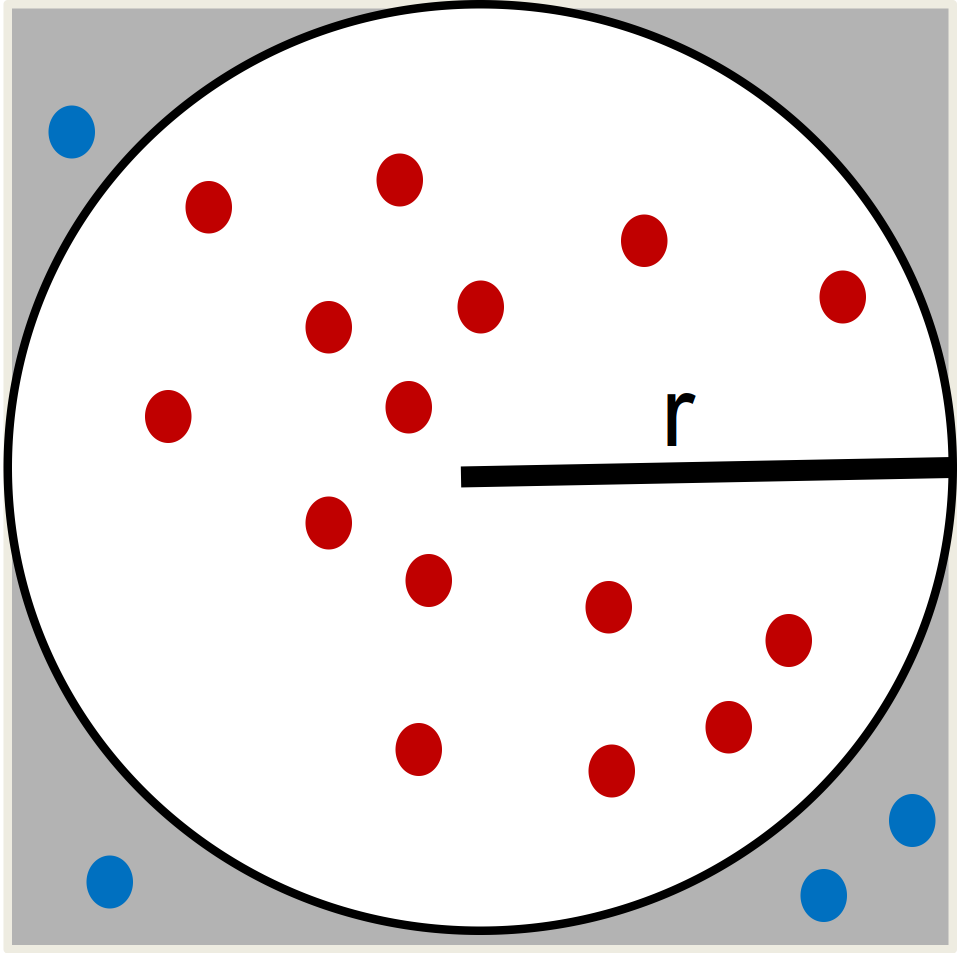
\includegraphics[width=1\textwidth]{pictures/montecarlopi}
	\end{minipage}
	$\pi = \frac{4*K}{N}$
\end{example}

\subsection{Diskrete Ereignissimulation}
